\documentclass{article}
\usepackage{geometry}
\geometry{
 a4paper,
 total={170mm,257mm},
 left=20mm,
 top=20mm,
 }
\usepackage{fontspec}

\usepackage{xunicode}

\usepackage{xltxtra}
\usepackage{indentfirst}

\usepackage{biblatex}
\addbibresource{fst.bib}

\usepackage{listings}

\usepackage{tikz}
\usetikzlibrary{shapes.geometric}

\setromanfont{SimSun}

\XeTeXlinebreaklocale “zh”
\XeTeXlinebreakskip = 0pt plus 1pt minus 0.1pt

\newcommand\Helvetica{\fontspec {Helvetica}}

\begin{document}
\title{FST}
\author{周乐钦}
\date{2015年12月10日}
\maketitle	

\section{导论}


\section{FST依赖的类}
org.apache.lucene.util.fst.BytesStore

org.apache.lucene.util.fst.Outputs

org.apache.lucene.util.packed.PackedInts.Reader

org.apache.lucene.util.fst.FST.Arc

org.apache.lucene.util.packed.GrowableWriter

org.apache.lucene.store.DataInput

org.apache.lucene.codecs.CodecUtil

org.apache.lucene.util.fst.BytesReader

org.apache.lucene.util.packed.PackedInts

org.apache.lucene.store.RAMOutputStream

org.apache.lucene.store.OutputStreamDataOutput

org.apache.lucene.store.InputStreamDataInput

\begin{center}
    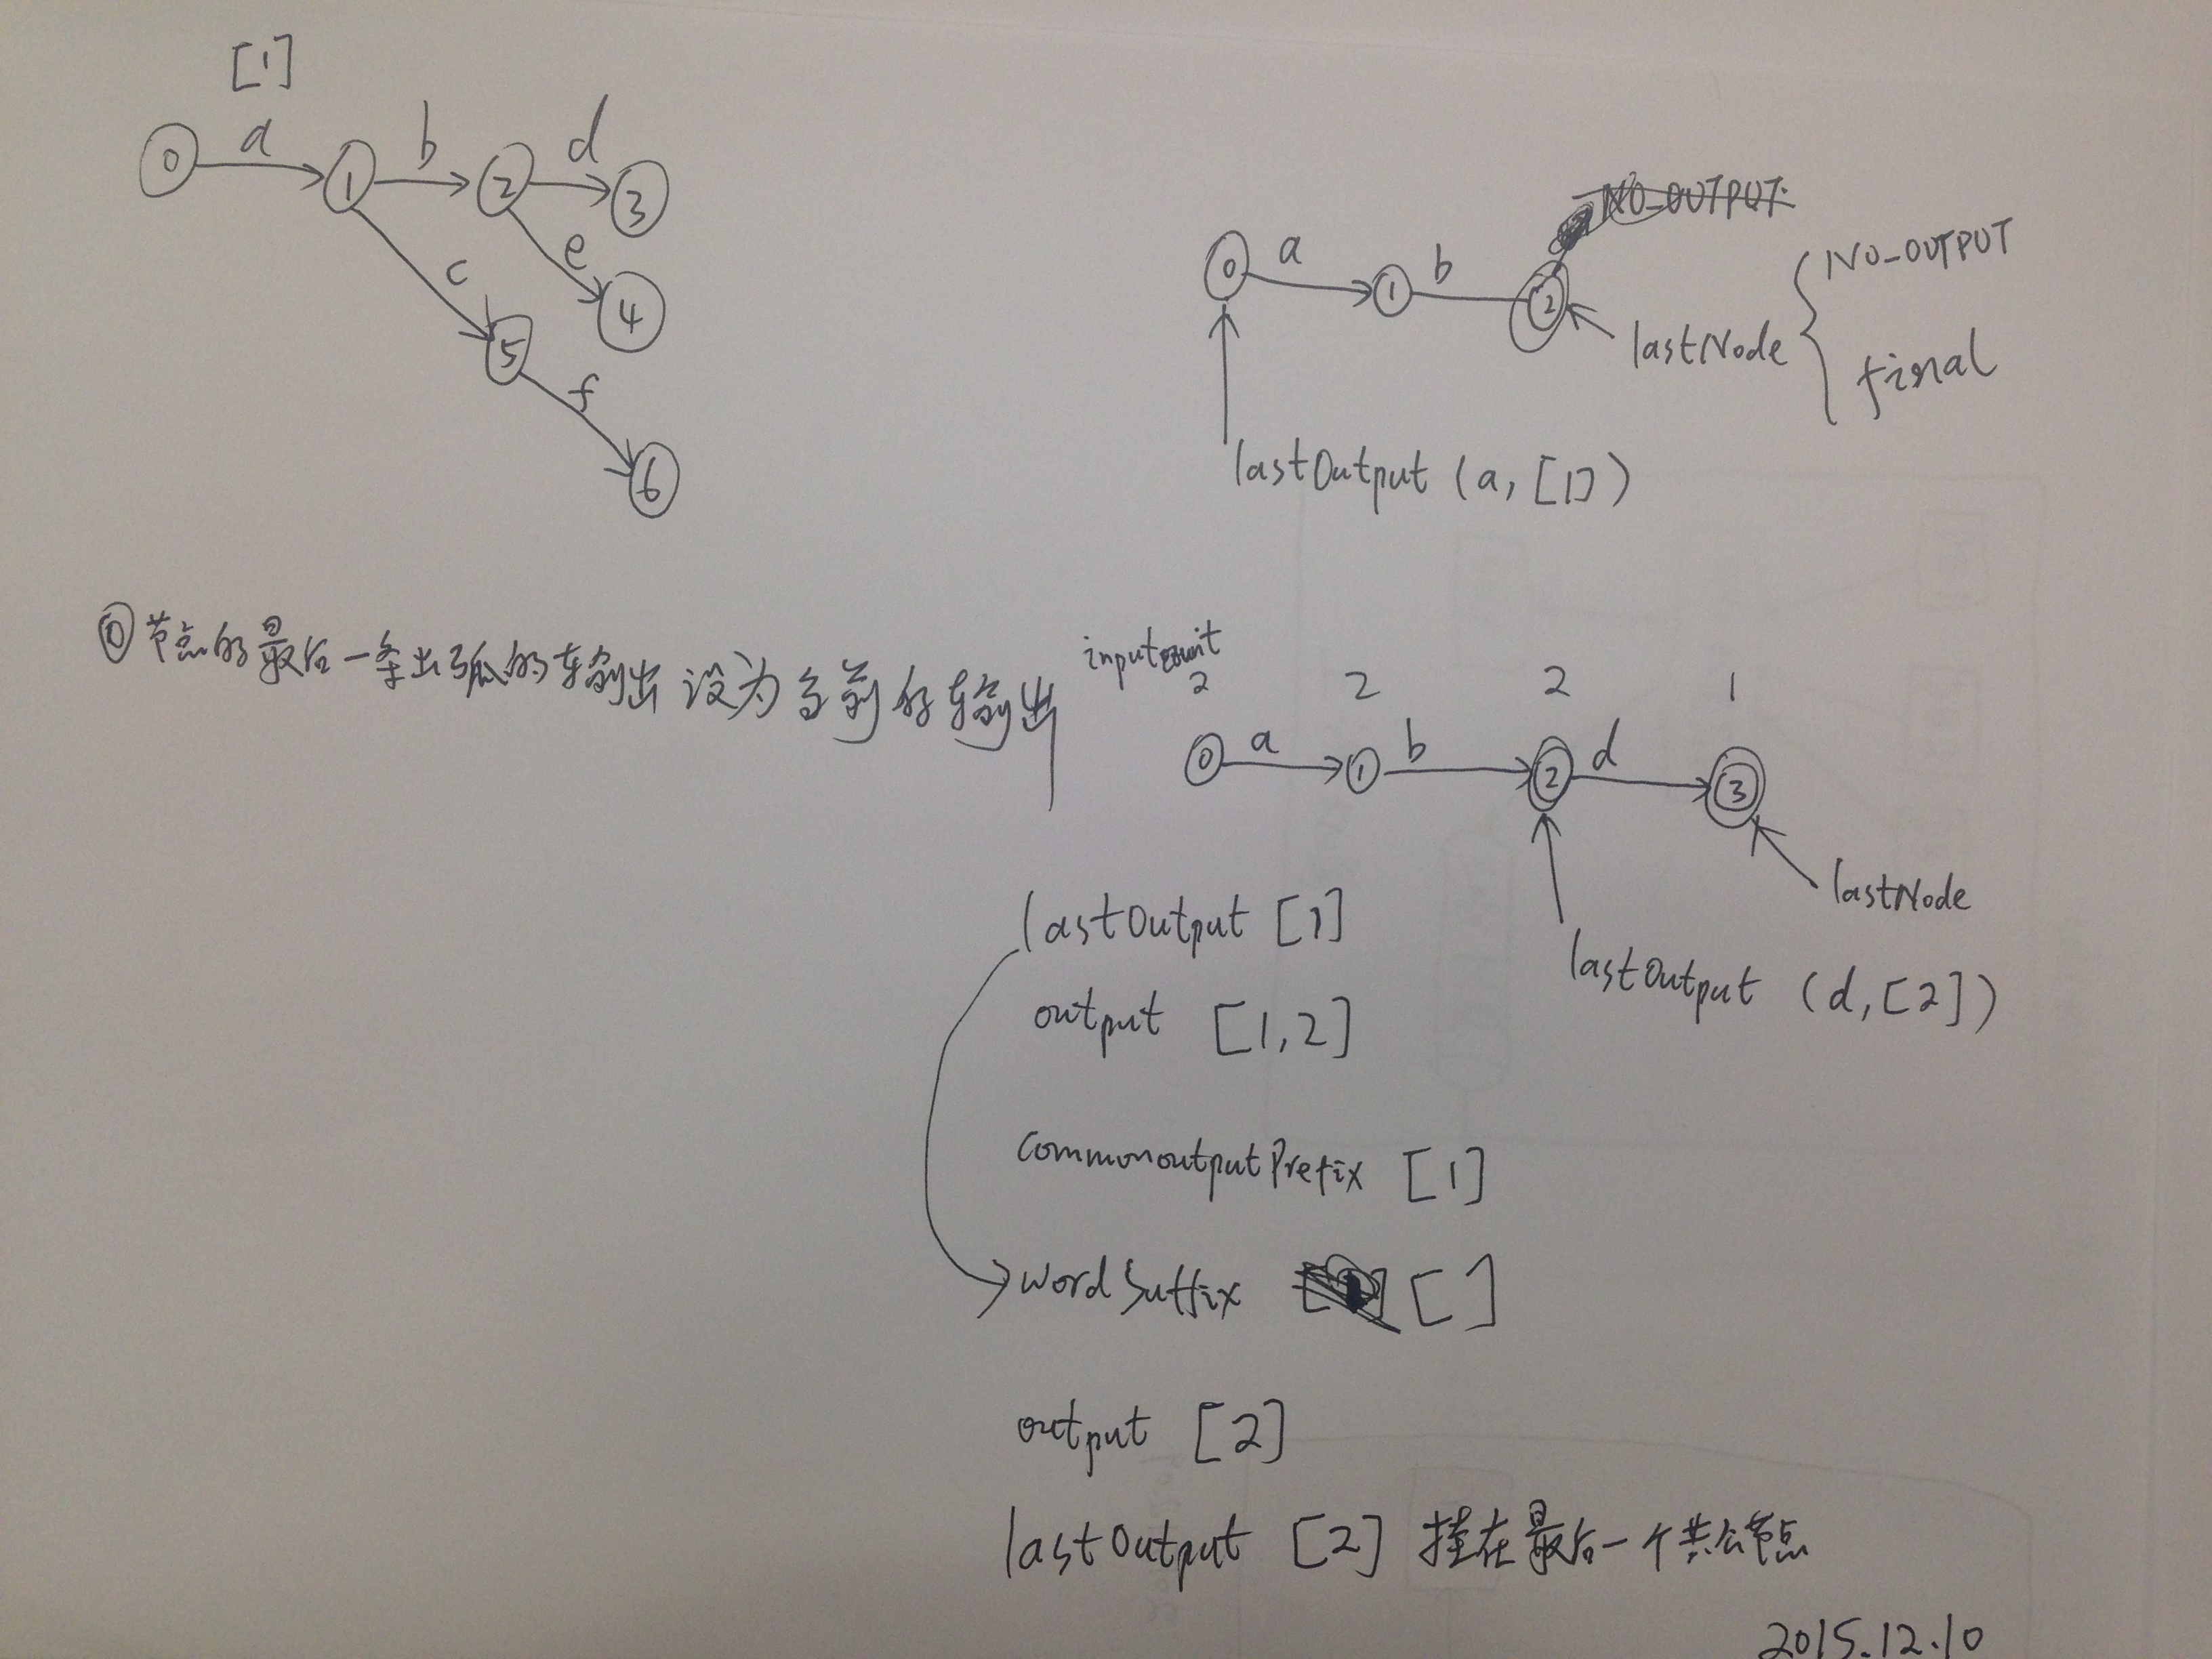
\includegraphics[width=360pt]{IMG_2809.JPG}
\end{center}

\begin{center}
    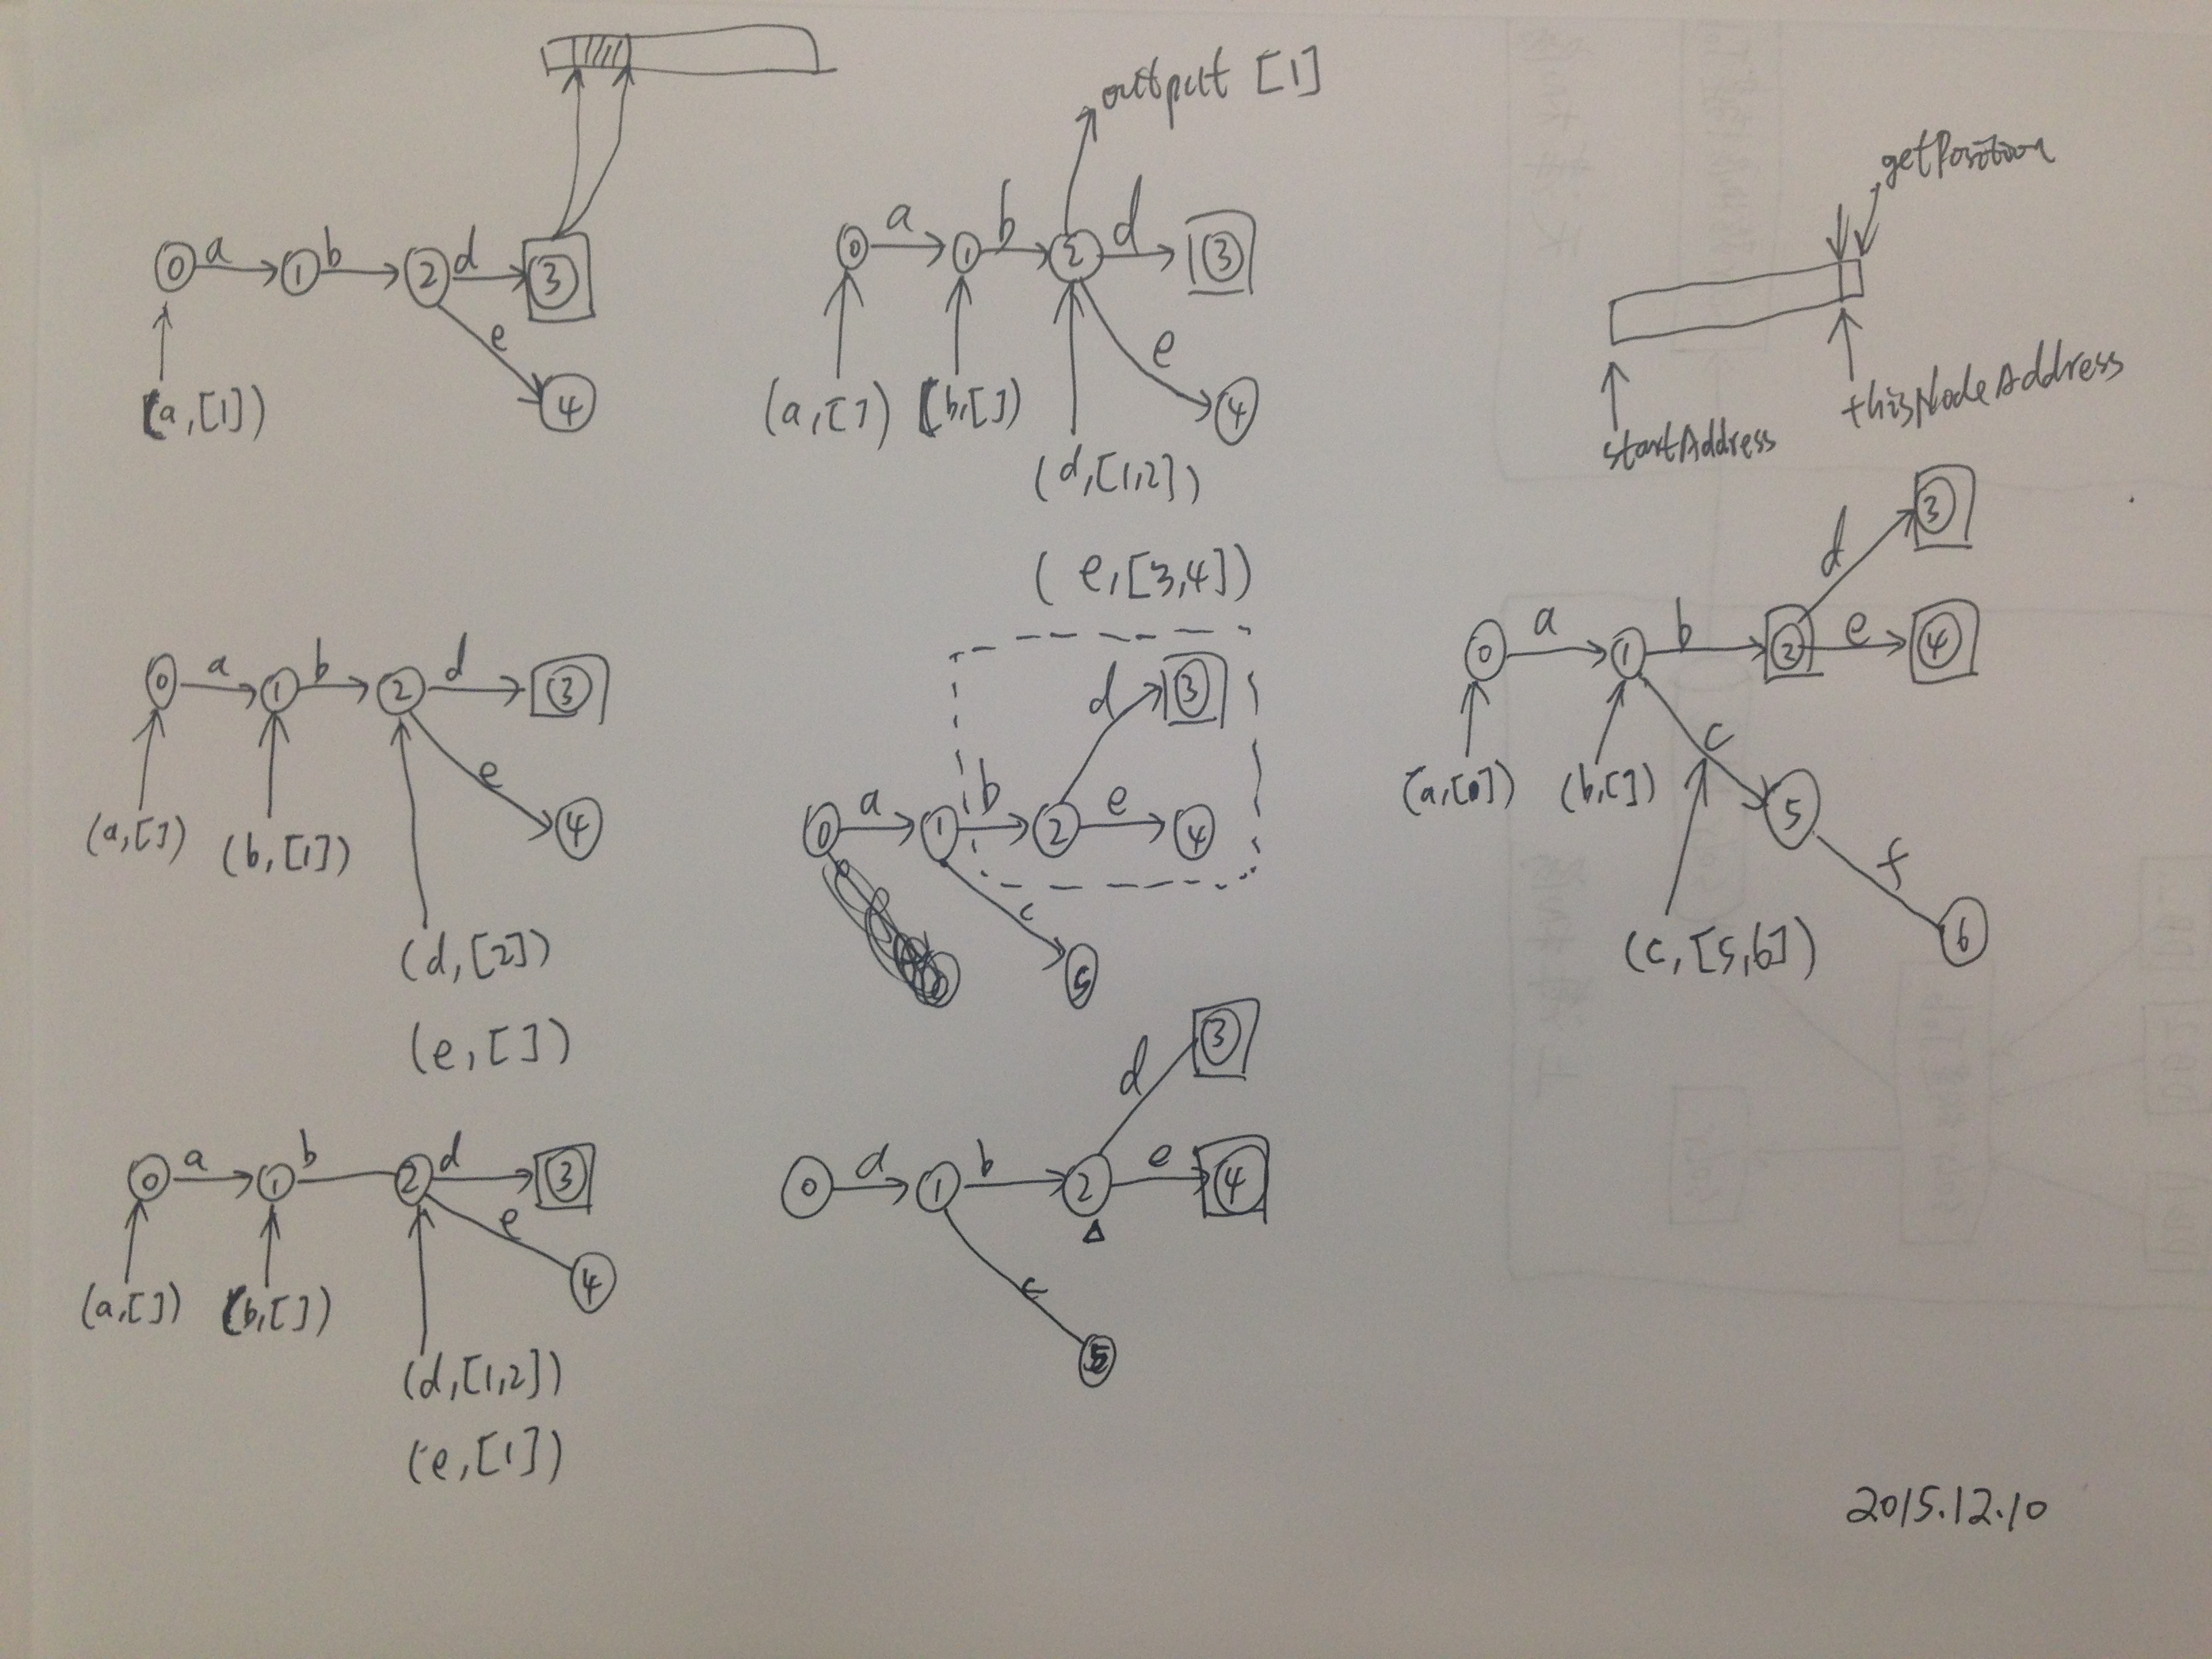
\includegraphics[width=360pt]{IMG_2810.JPG}
\end{center}


\section{INPUT\_TYPE}

枚举值 {BYTE1, BYTE2, BYTE4}

\section{常量}
BIT\_FINAL\_ARC 1 0b1

BIT\_LAST\_ARC 2 0b10

BIT\_TARGET\_NEXT 4 0b100

BIT\_STOP\_NODE 8 0b1000

BIT\_ARC\_HAS\_OUTPUT 16 0b10000

BIT\_ARC\_HAS\_FINAL\_OUTPUT 32 0b100000

BIT\_TARGET\_DELTA 64 0b1000000

BIT\_TARGET\_DELTA 128 0b10000000

ARCS\_AS\_FIXED\_ARRAY = BIT\_ARC\_HAS\_FINAL\_OUTPUT

FIXED\_ARRAY\_SHALLOW\_DISTANCE 3

FIXED\_ARRAY\_NUM\_ARCS\_SHALLOW 5

FIXED\_ARRAY\_NUM\_ARCS\_DEEP 10

\section{版本相关常量}
VERSION\_START = 0

VERSION\_INT\_NUM\_BYTES\_PER\_ARC = 1

VERSION\_SHORT\_BYTE2\_LABELS = 2

VERSION\_PACKED = 3

VERSION\_VINT\_TARGET = 4

VERSION\_NO\_NODE\_ARC\_COUNTS = 5

VERSION\_CURRENT = VERSION\_NO\_NODE\_ARC\_COUNTS


\section{Builder}

\subsection{配置型字段说明}

\subsubsection{剪枝}

Yes, BlockTreeTermsWriter uses freezeTail to figure out where to draw
the lines for assigning terms to blocks, but to build the trie terms
index it builds a separate FST, by adding in each block's prefix (it
doesn't use the FST's builder pruning to create the trie).


When you turn on pruning, FST Builder will just remove nodes that don't have a high enough count of input terms traversing through them. E.g. if minSuffixCount1 is 100 then only FST nodes that see >= 100 input terms coming through them, are preserved. You can use this to build a prefix trie instead of the full FST. Creating a custom tail freezer is very expert: it lets you implement arbitrary logic on which nodes are pruned or not\cite{lucene-fst-prune, lucene-fst-prune-2}.

\textbf{[minSuffixCount1]}

简单剪枝。如果一个节点少于minSuffixCount1个项通过它,我们剪掉这个节点及所有尾随节点。

\textbf{minSuffixCount2}

更好的剪枝。如果一个节点的前节点少于minSuffixCount2个项通过他,我们剪掉这个节点及所有尾随节点。

\subsubsection{共享后缀}
\textbf{doShareSuffix}

将共享的后缀合成一个唯一后缀路径。FST更小,但在构建时消耗更多的内存和CPU。

\textbf{doShareNonSingletonNodes}

仅在doShareSuffix成立时有效,确保FST完全最小化,消耗更多的CPU和内存。

\textbf{shareMaxTailLength}

仅在doShareSuffix成立时有效,设置成Integer.MAX\_VALUE确保FST完全最小化,消耗更多的CPU和内存。

\subsubsection{紧凑打包}

\textbf{doPackFST}

创建一个紧凑打包的FST

\textbf{acceptableOverheadRatio}

creates an FST by packing this one.  This up to ~8 bytes per node depending on process requires substantial additional RAM (currently <code>acceptableOverheadRatio</code>), but then should produce a smaller FST. The implementation of this method uses ideas from Smaller Representation of Finite State Automata\cite{daciuk2011smaller}which describes techniques to reduce the size of a FST. However, this is not a strict implementation of the algorithms described in this paper.

创建GrowableWriter类型的nodeAddress

创建GrowableWriter类型的inCounts

\begin{tikzpicture}
	%Node
\node[draw,diamond,aspect=4,text width=12em] {This is a test for diamond};

\end{tikzpicture}

\subsubsection{弧存储}

\textbf{allowArrayArcs}

允许使用数组存储弧,优化遍历速度

\section{Builder的构造函数}

public Builder(FST.INPUT\_TYPE inputType, int minSuffixCount1, int minSuffixCount2, boolean doShareSuffix,
                 boolean doShareNonSingletonNodes, int shareMaxTailLength, Outputs<T> outputs,
                 boolean doPackFST, float acceptableOverheadRatio, boolean allowArrayArcs,
                 int bytesPageBits)
                 
可以设置所有配置。

public Builder(FST.INPUT\_TYPE inputType, Outputs<T> outputs);

使用默认配置。

仅在doPackFST成立时有效,紧凑打包FST时怎样权衡速度和空间。参考PackedInts\#getMutable(int, int, float)。

\setlength{\unitlength}{0.8cm}
\begin{picture}(12,4)
\thicklines
\put(8,3.3){{\footnotesize $3$-simplex}}
\put(9,3){\circle*{0.1}}
\put(8.3,2.9){$a_2$}
\put(8,1){\circle*{0.1}}
\put(7.7,0.5){$a_0$}
\put(10,1){\circle*{0.1}}
\put(9.7,0.5){$a_1$}
\put(11,1.66){\circle*{0.1}}
\put(11.1,1.5){$a_3$}
\put(9,3){\line(3,-2){2}}
\put(10,1){\line(3,2){1}}
\put(8,1){\line(1,0){2}}
\put(8,1){\line(1,2){1}}
\put(10,1){\line(-1,2){1}}
\end{picture}

\section{方法}

\subsection{add}

public void add(IntsRef input, T output) throws IOException;


计算上一个输入和当前输入的公共前缀

pos1指向lastInput的下标,下标指向元素不属于公共前缀

pos2指向input的下标


2.1 Arc

弧上面的标签

弧指向的节点

弧上的输出

弧是否为最终的弧

2.2 UnCompiledNode

拥有者

指向这个节点的弧的数量inputCount

从此节点发出的弧arcs


long FST::addNode(Builder<T> builder, Builder.UnCompiledNode<T> nodeIn) throws IOException;

调用private boolean shouldExpand(Builder<T> builder, UnCompiledNode<T> node)方法得到条件doFixedArray

固定数组消耗更多的内存,但是可以在按弧标签搜索弧时采用二分搜索算法而不是线性扫描算法。

Builder的arcCount记录总的弧数量

依次处理节点的出弧

每个弧,设置它的flags

BIT\_LAST\_ARC 从节点出去的最后一条弧

BIT\_TARGET\_NEXT 最后冻结的节点与弧指向的节点相同且不用固定数组

BIT\_FINAL\_ARC 最终的弧

BIT\_ARC\_HAS\_FINAL\_OUTPUT 有最终输出

BIT\_STOP\_NODE 指向的节点是最终节点

BIT\_ARC\_HAS\_OUTPUT 弧上没有输出

【数据写入】写入flags(一个字节)

【数据写入】写入弧上的标签(传入类型为整数,实际占用字节数按条件定)

INPUT\_TYPE.BYTE1 一个字节

INPUT\_TYPE.BYTE2 两个字节

INPUT\_TYPE 为其他 变长编码

【数据写入】写入弧上的输出

【writeVInt】变长编码保存长度

【writeBytes】字节数组保存实际内容

【数据写入】写入弧上的最终输出

ByteSequenceOutputs类型输出

【writeVInt】变长编码保存长度

【writeBytes】字节数组保存实际内容

如果指向的目标点有弧且标记没有BIT\_TARGET\_NEXT

【数据写入】指向的目标节点的hash值

【writeVLong】变长长整形编码


如果是采用固定数组,计算当前弧占用的字节数、更新最后弧结束位置lastArcStart,更新弧所占字节数的最大值maxBytesPerArc

翻转弧的字节

Builder节点总数nodeCount加1

返回节点的地址thisNodeAddress,翻转之前最后一个字节的地址,翻转之后第一个字节的地址


public long NodeHash::add(Builder<T> builder, Builder.UnCompiledNode<T> nodeIn) throws IOException

计算节点的hash值

调用long FST::addNode(Builder<T> builder, Builder.UnCompiledNode<T> nodeIn) throws IOException;保存节点到FST

记录在hash表,key为hash值,value为添加的节点的地址

返回节点的地址


private CompiledNode Builder::compileNode(UnCompiledNode<T> nodeIn, int tailLength) throws IOException

把节点添加到NodeHash表

记录最后一次记录的节点地址到lastFrozenNode

清除nodeIn

创建CompiledNode,它的字段node保存NodeHash的add函数返回的节点地址

返回CompiledNode对象

\subsubsection{共享后缀}

构造Builder时设置doShareSuffix,如果设置为true,则创建一个NodeHash类型的dedupHash


\section{Builder完成}

public FST<T> Builder::finish() throws IOException;

获取frontier的第一个节点

调用Builder的private void freezeTail(int prefixLenPlus1) throws IOException方法,传入0,即从第一个节点开始冻结

调用FST的 void finish(long newStartNode) throws IOException 方法,结束本次FST构建

\section{FST}

\subsection{FST构建完成}

void FST::finish(long newStartNode) throws IOException;



调用FST的private void cacheRootArcs() throws IOException方法第一层的之多128个标签

\begin{center}
    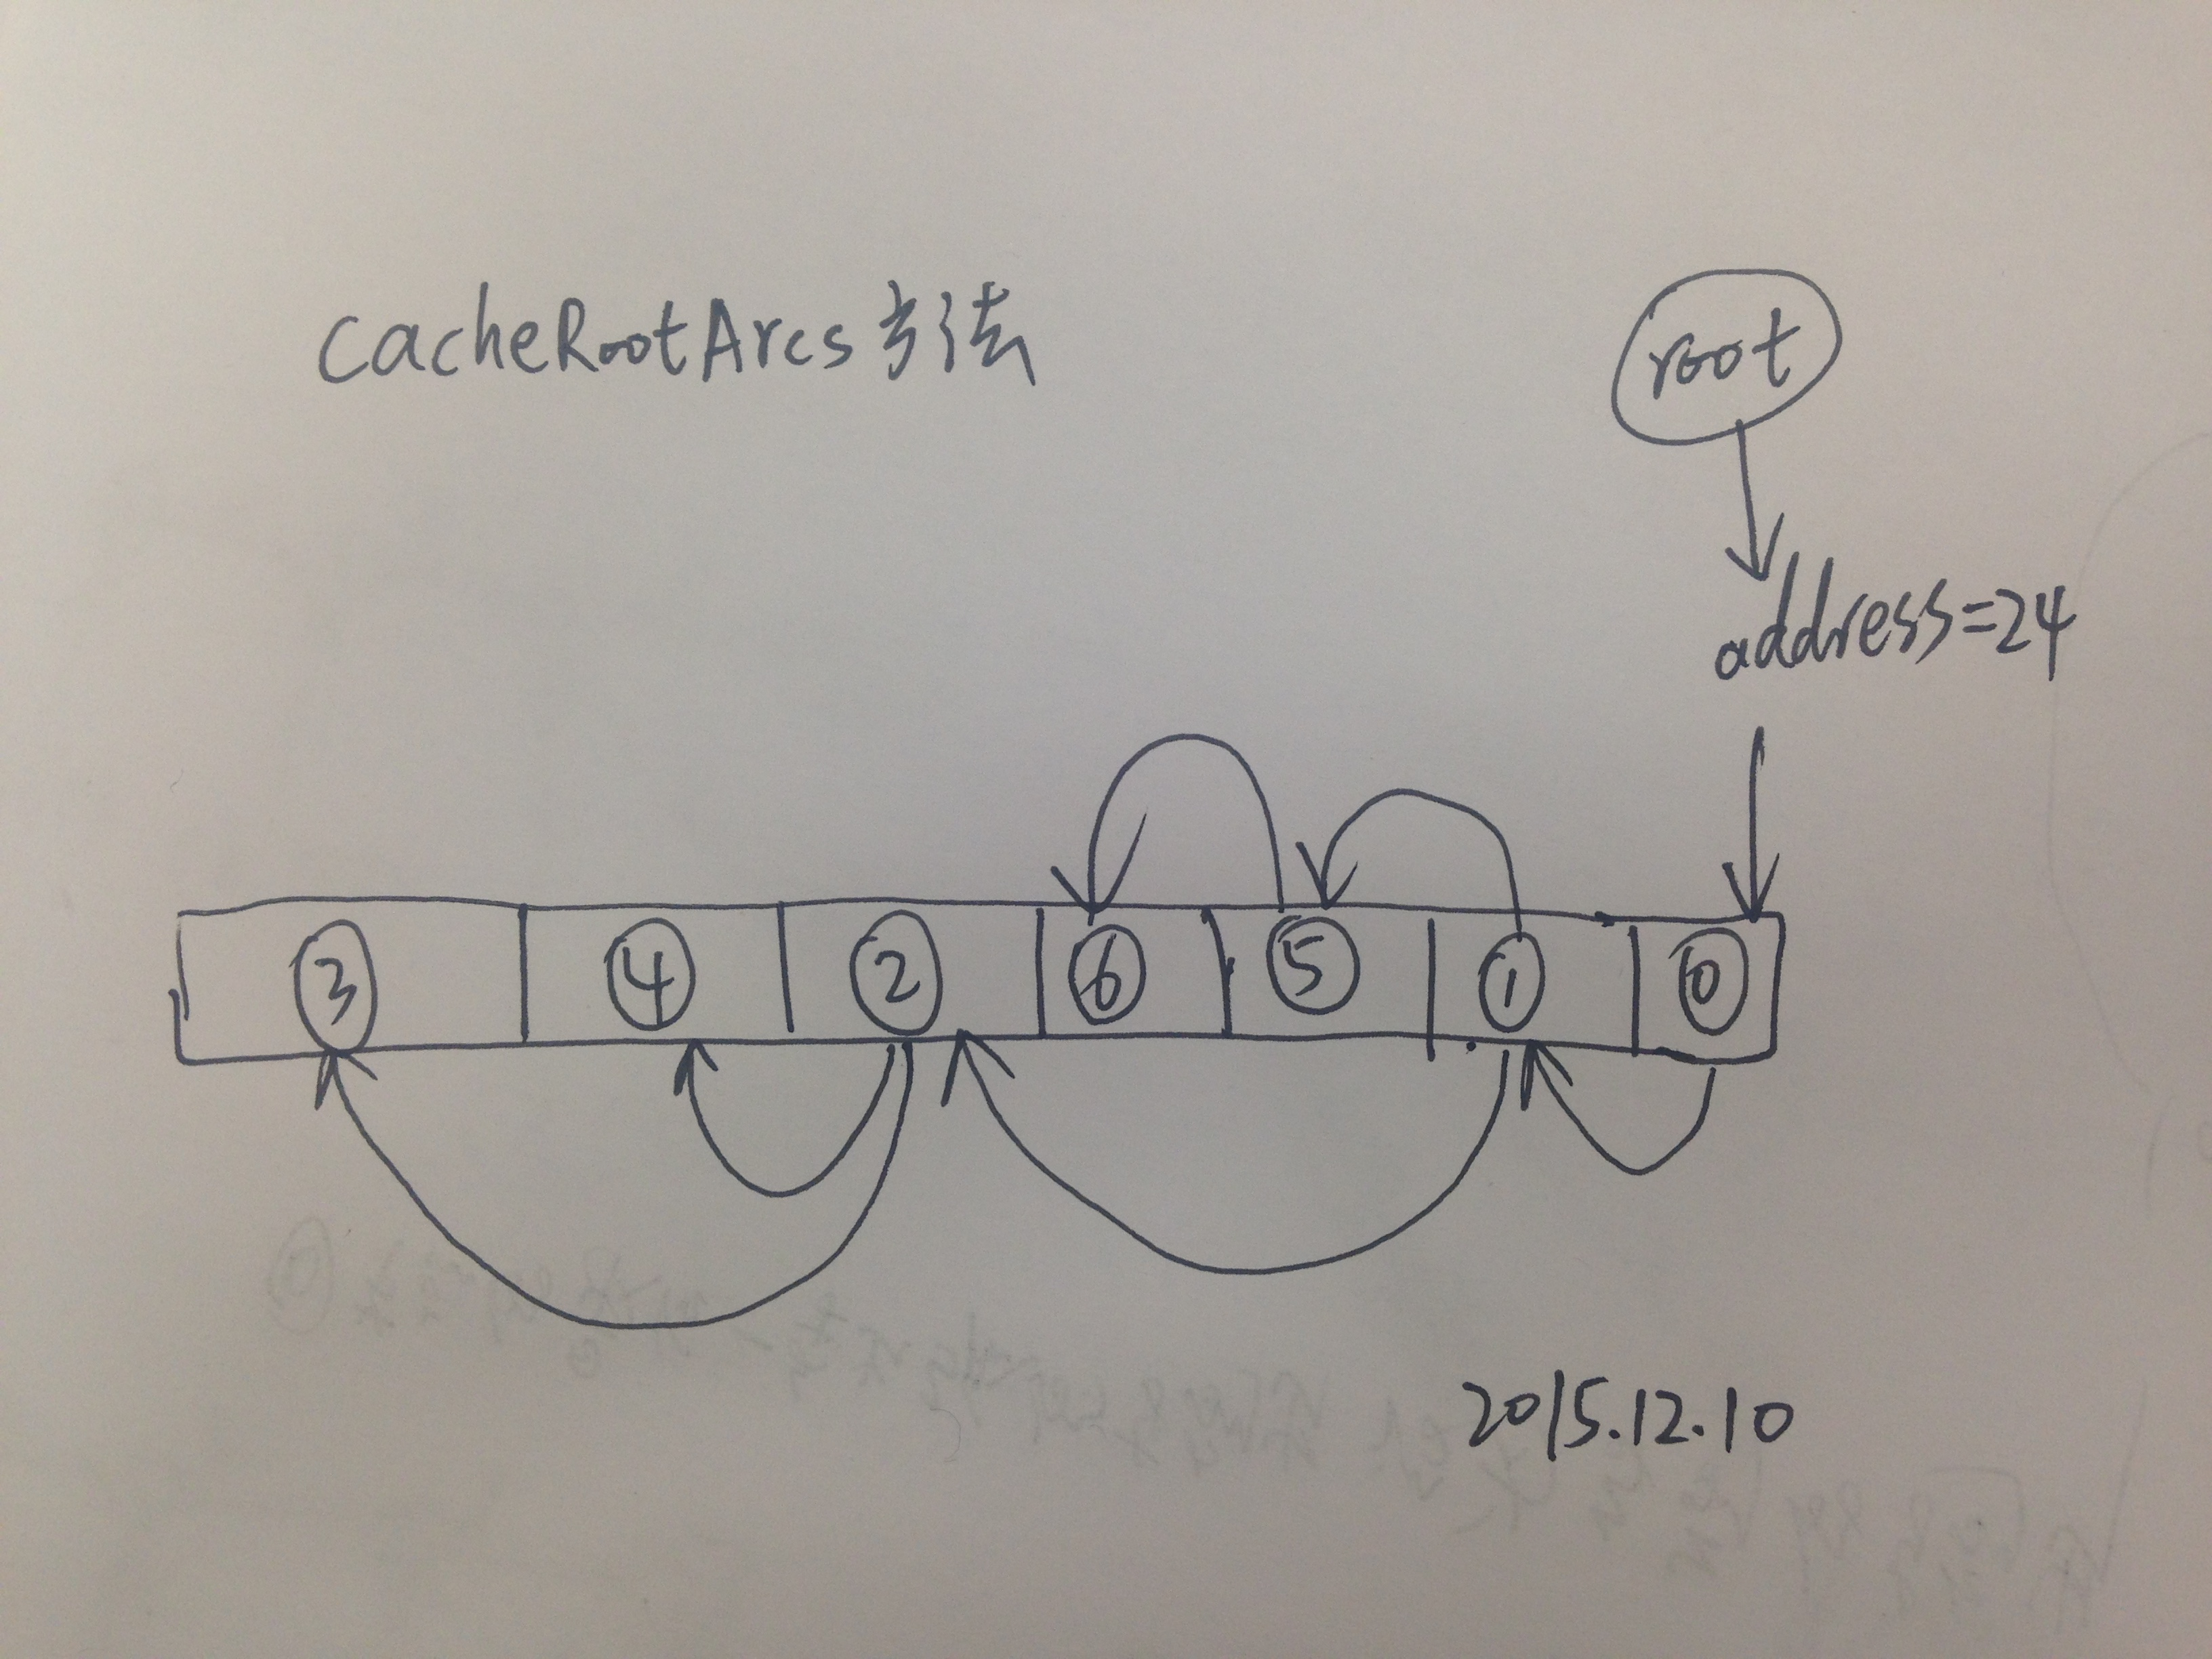
\includegraphics[width=480pt]{IMG_2811.JPG}
\end{center}

cacheRootArcs调用getFirstArc方法

\subsection{getFirstArc}

创建一个虚拟的弧,指向第一个真实的节点

target=24

cacheRootArcs调用readFirstRealTargetArc方法读取真实的第一个弧

\subsection{pack}

FST<T> FST::pack(Builder<T> builder, int minInCountDeref, int maxDerefNodes, float acceptableOverheadRatio) throws IOException;

minInCountDeref 最小的入弧数量

minInCountDeref = 3

maxDerefNodes 最大节点数

maxDerefNodes = 10

inCounts 记录每个节点的入弧数量,初始容量大小为8

\begin{enumerate}
	\item 计算需要保存多少个入弧数量靠前的节点,创建topN大小的优先级队列NodeQueue
	\item Map<Integer,Integer>关联数组topNodeMap,键为node,值为优先级队列中从后往前数得到的索引位置
	\item 创建GrowableWriter类型的newNodeAddress,第一个参数为node地址值需要的字节数,第二个参数为节点数量再加一,第三个参数为可接受的overhead比率
	\item 粗粒度猜测地址后填充到newNodeAddress,索引为每个节点的编号,从1开始;值为占用的空间大小,字节数
	\item 一个while true循环
	\begin{enumerate}
		\item 创建一个packed FST,bytesPageBits=1
			\paragraph{}
			[write] 写入字节类型的0,目的是跳过0,因为0是保留的目标节点
			\paragraph{}
			absCount = 0
			\paragraph{}
			deltaCount = 0
			\paragraph{}
			topCount = 0
			\paragraph{}
			nextCount = 0
			\begin{enumerate}
				\item 循环处理每个一个节点
					\paragraph{}
					因为我们反转了字节,所以从最后一个字节开始处理
					\begin{enumerate}
						\item 循环尝试写入节点
						\paragraph{}
						从原fst读取第一条弧
						\item 循环处理这个节点的每条弧
						\paragraph{}
						对目标节点的存储使用差值编码
					\end{enumerate}
			\end{enumerate}
	\end{enumerate}
\end{enumerate}
\section{FST get}

public static<T> T Util::get(FST<T> fst, BytesRef input) throws IOException


获取虚拟的弧

调用FST的public Arc<T> findTargetArc(int labelToMatch, Arc<T> follow, Arc<T> arc, BytesReader in) throws IOException方法

follow当前的弧,根据当前的弧指向的节点,查找从那个节点射出的弧,如果某个弧上的标签与输入的字符串中当前处理的字符相等,则找到匹配的弧;下一次用这个新的弧作为follow弧进行下一次搜索

\begin{center}
    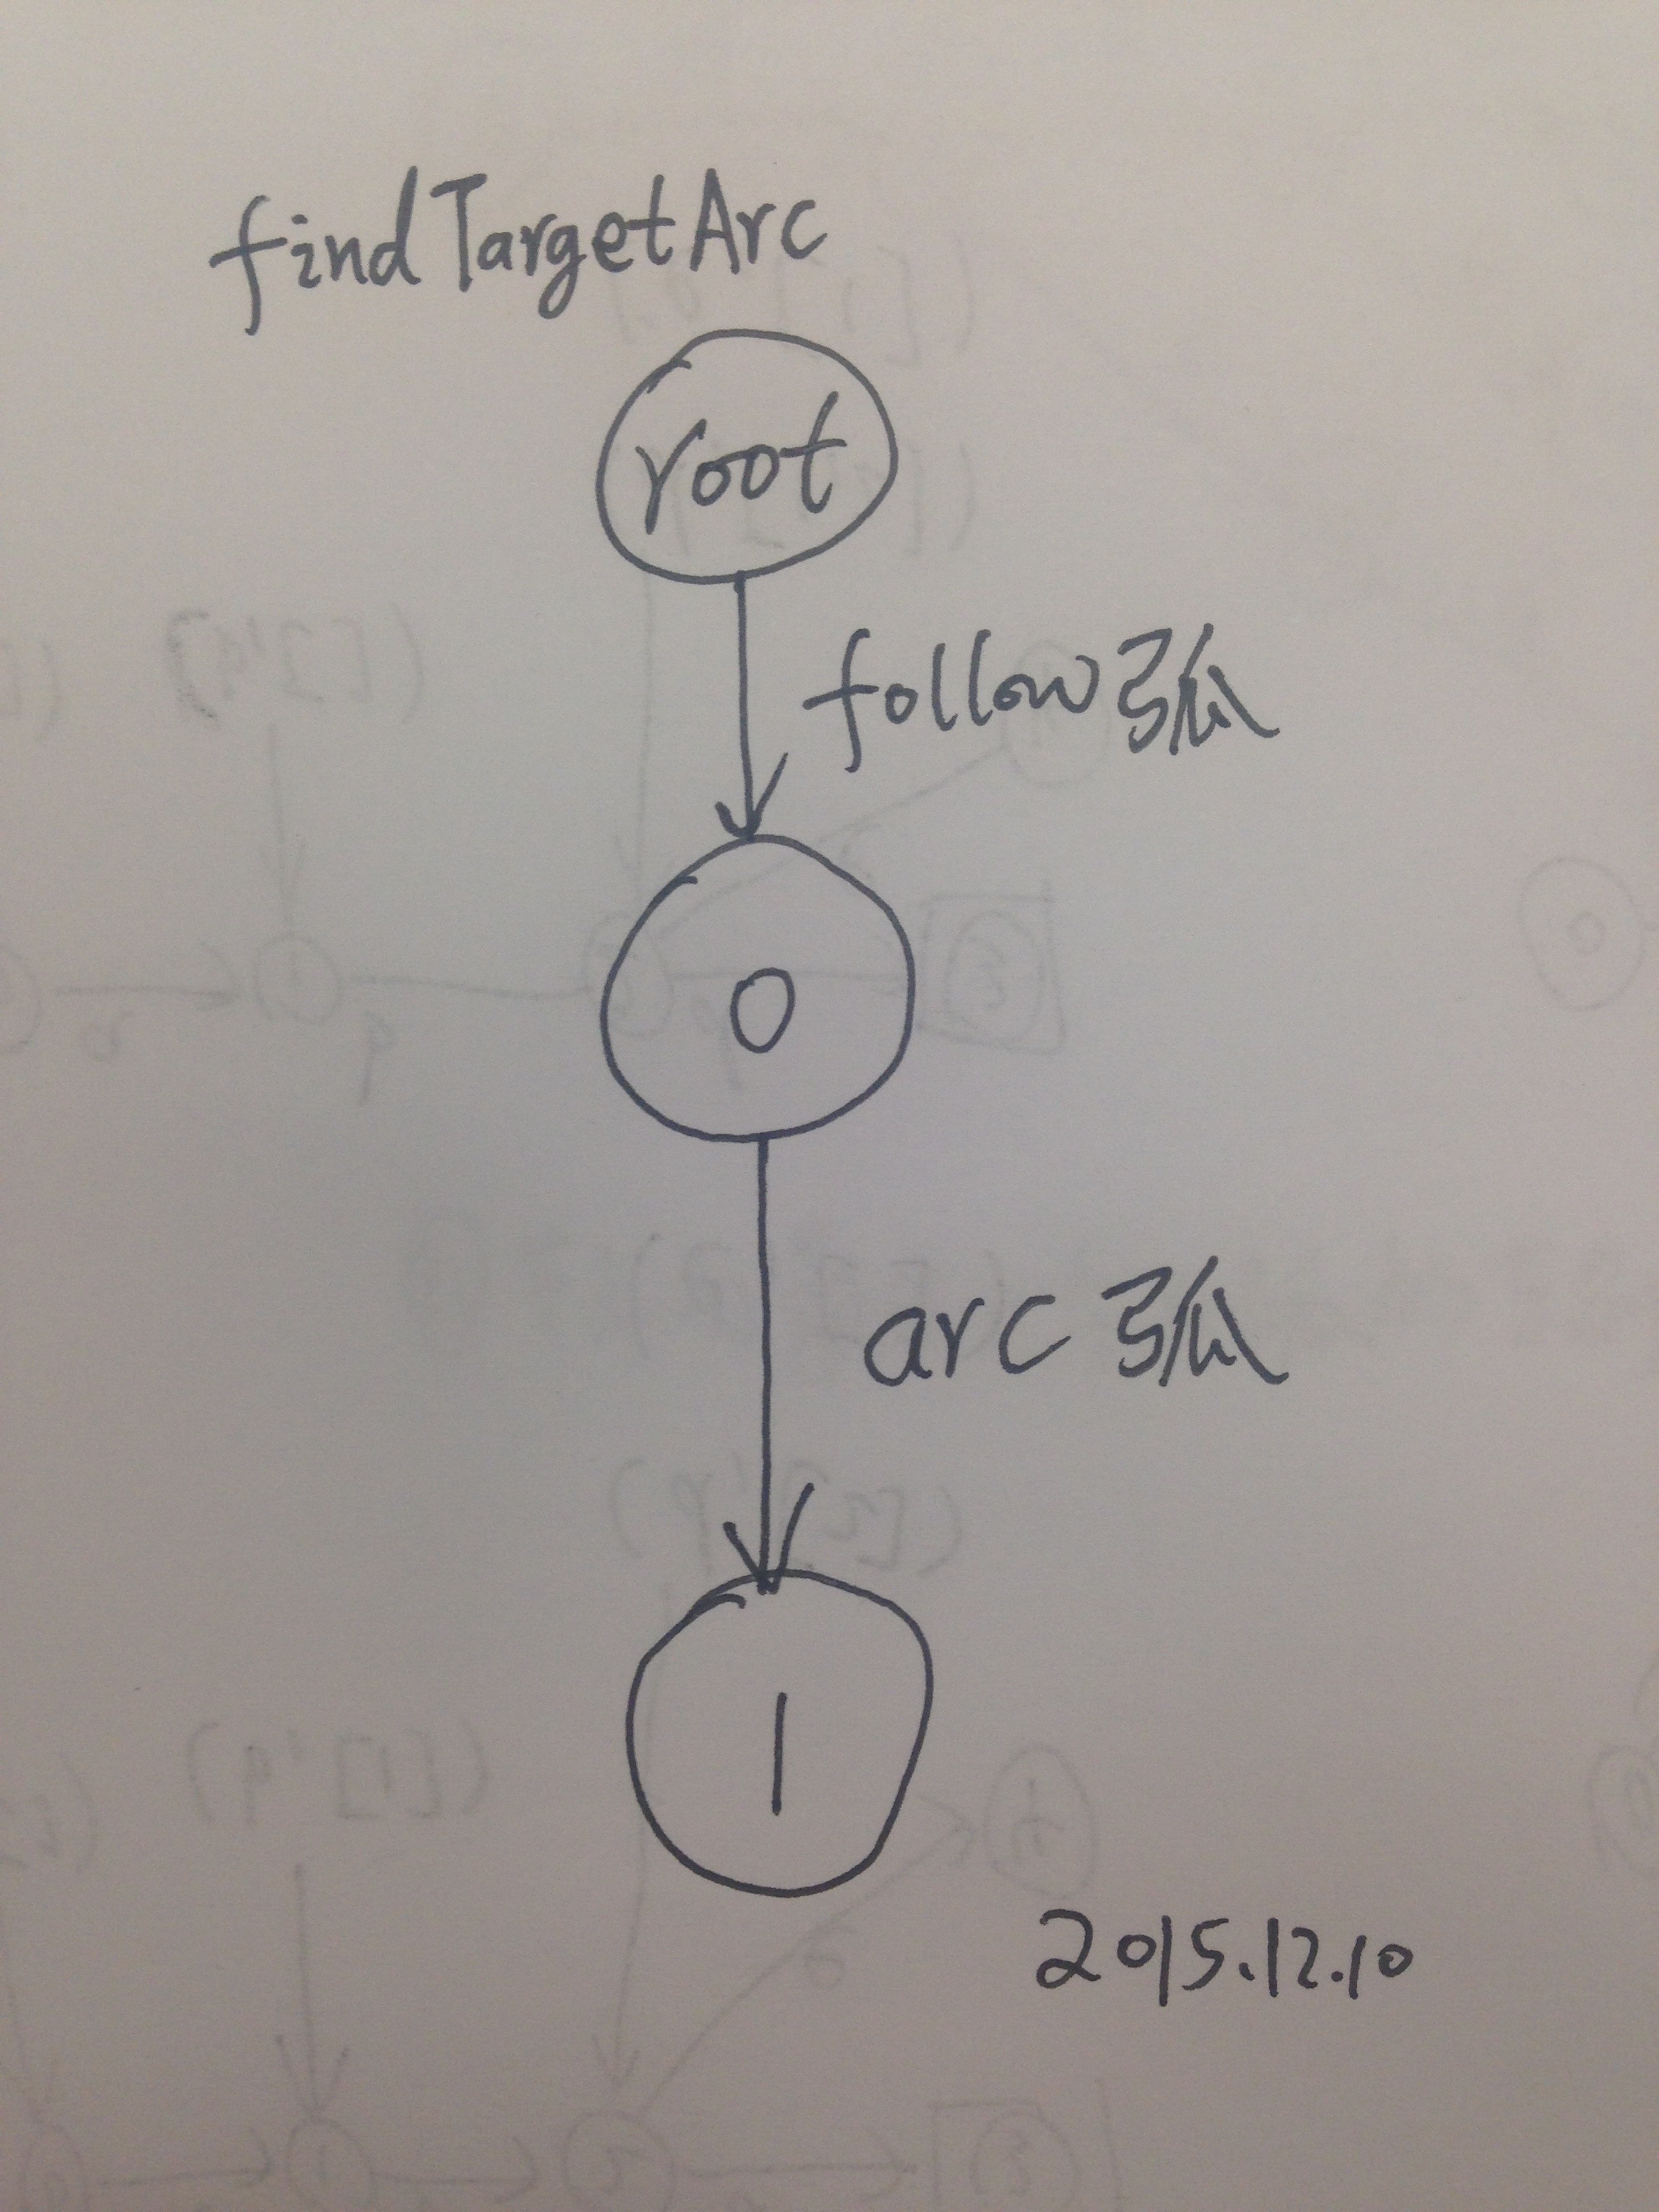
\includegraphics[width=480pt]{IMG_2012.jpg}
\end{center}

\section{延伸阅读}
http://web.cs.mun.ca/~harold/Courses/Old/CS4750.F14/Diary/fla.pdf

http://cs.nyu.edu/~mohri/pub/fst.pdf

http://openfst.org/twiki/pub/FST/FstHltTutorial/tutorial_part1.pdf

http://openfst.org/twiki/pub/FST/FstHltTutorial/tutorial_part2.pdf

http://openfst.org/twiki/pub/FST/FstHltTutorial/tutorial_part3.pdf

\printbibliography

\end{document}
